\section{Graphical Design}\label{GraphicalDesign}
In graphical design, like in any other design, there are many options to be considered. Colours, fonts, balance and many more factors should be considered and chosen carefully. Most importantly, how to mix these elements together without making a mess. 
This will reflect greatly on how a design is being perceived. \cite{ColorMeaning}

\subsubsection{Colours}\label{Colours}

Colours are more than just colours when designing a brand, an app or a website. Colours are perceived in various ways and are a big part of how the design is coming across to the user. \cite{ColorMeaning}

It is important to remember that when choosing the colour palette for a design, how we perceive colour is very different. Also, colours can change according to what is next to them. Yellow might look different next to grey than it will look next to purple for instance. \cite{ColorMeaning}

When it comes to colour psychology the truth is, it is too dependent on personal experience. There is no right answer to which colour that represents a certain feeling. \cite{ColorMeaning}
There are many studies conducted on this matter. 
One study shows that 90\% of people make snap judgement based on colour alone. \cite{ColorMeaning} Another study shows that an intend of purchasing is linked with how a brand is perceived i.e. what kind of "personality" does the brand have?\cite{ColorMeaning}

\begin{figure}[H]
\centering
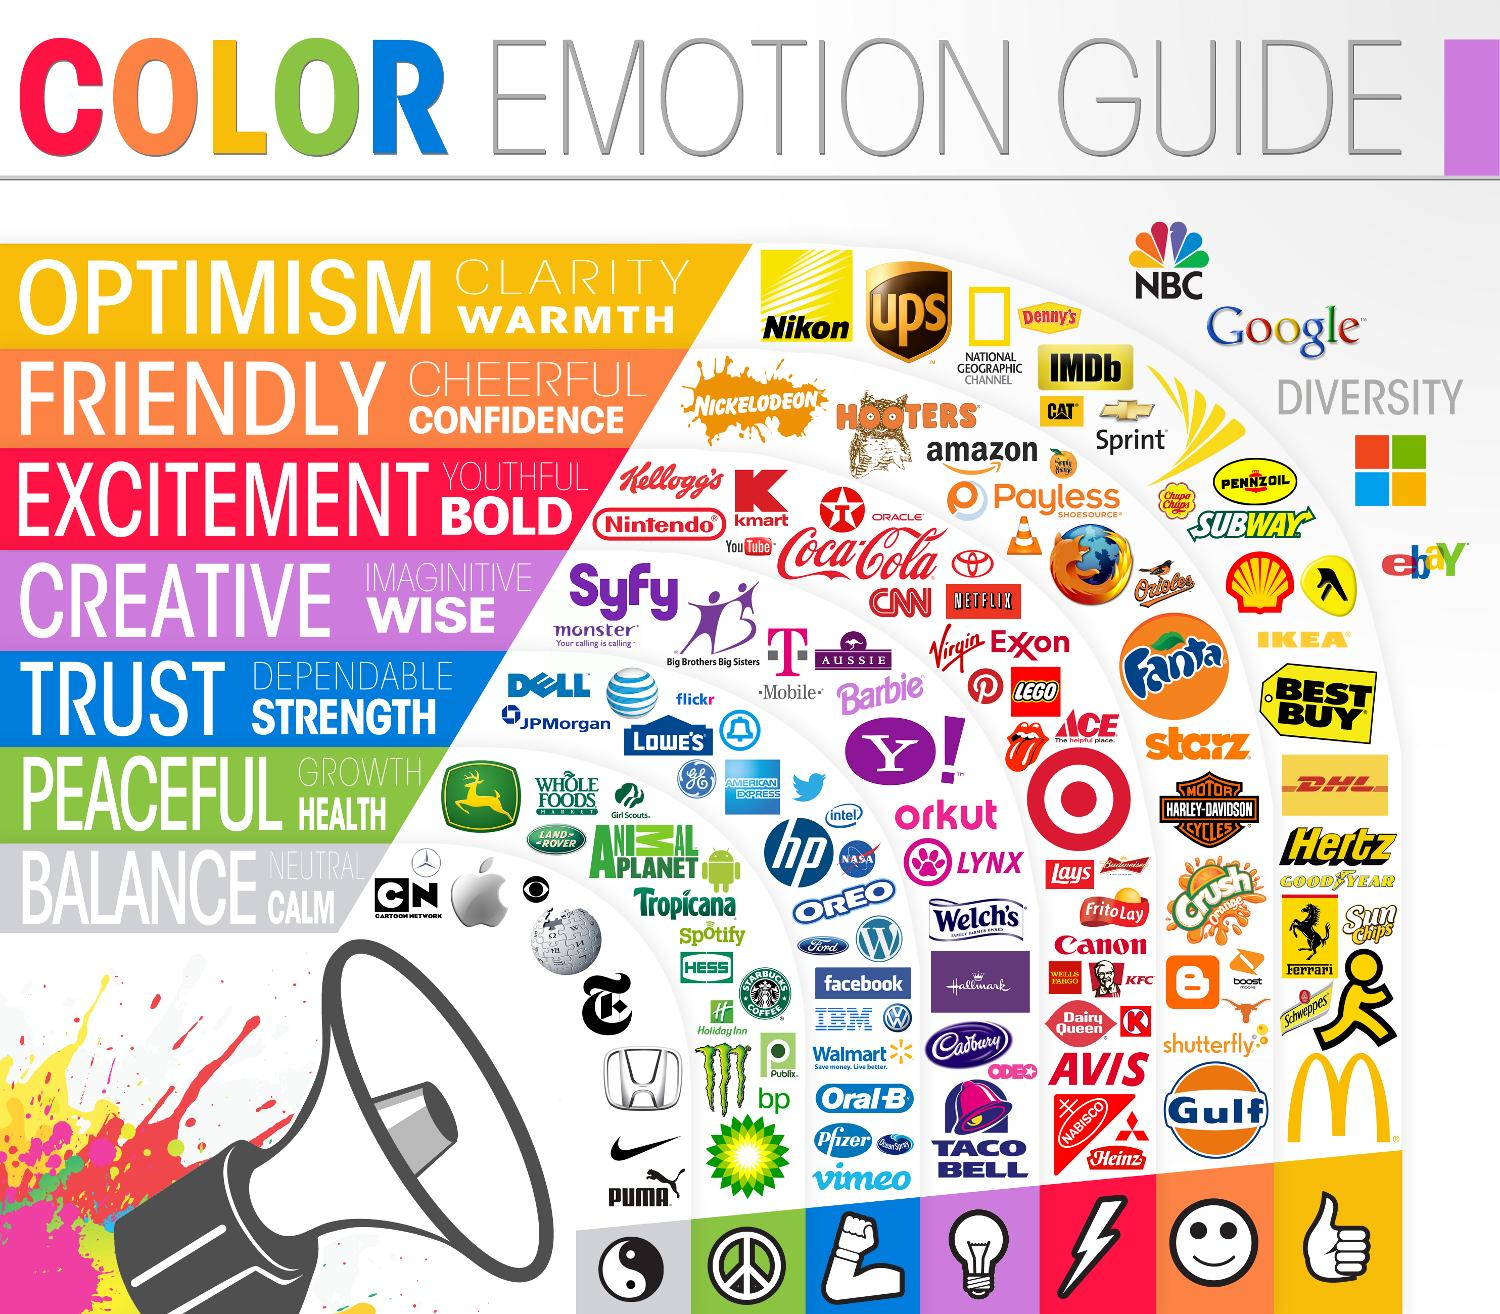
\includegraphics[scale=0.125]{color-emotion.jpg}
\caption{Overall image of how colours are generally perceived.} \cite{ColorMeaning}
\end{figure}

But all in all, the concept of the app is key. Many studies show that it is way more important to choose a colour that shows the personality of the product, rather than picking a stereotype colour. \cite{ColorMeaning}

So how does one find the best way to coordinate different colours? Research indicates that the isolation effect is very useful \cite{Normans}.

\begin{figure}[H]
\centering

\includegraphics[scale=0.5]{isolation_effect.png}
\caption{"The sign-up button stands out because it is like a red "island" in a sea of blue." \cite{ColorMeaning}}
\label{isolationFig}
\end{figure}

Using the isolation effect will help the user have a more efficient experience because the most important feature e.g. a "sign up" button (As shown in figure \ref{isolationFig}), stands out. \cite{ColorMeaning} 
Research suggests that a colour scheme that consists of analogue colours and combining it with an accent complimentary colour or a tertiary colour is preferred amongst users. \cite{ColorMeaning} 

When designing the layout it is key to keep everything simple and streamlined. 
Choosing a colour scheme should be done carefully. In general, the graphics should be kept clean and simple.